\documentclass{article}

\usepackage{graphicx}
\usepackage{booktabs}
\usepackage{longtable}
\usepackage{tabu}
\usepackage{listings}
\usepackage{hyperref}
\usepackage{tcolorbox}

\title{Dental image classification}

\author{%
elefun
}

\begin{document}

\maketitle

\section{Section 1}

\begin{figure}[!htb]
\minipage{0.49\textwidth}
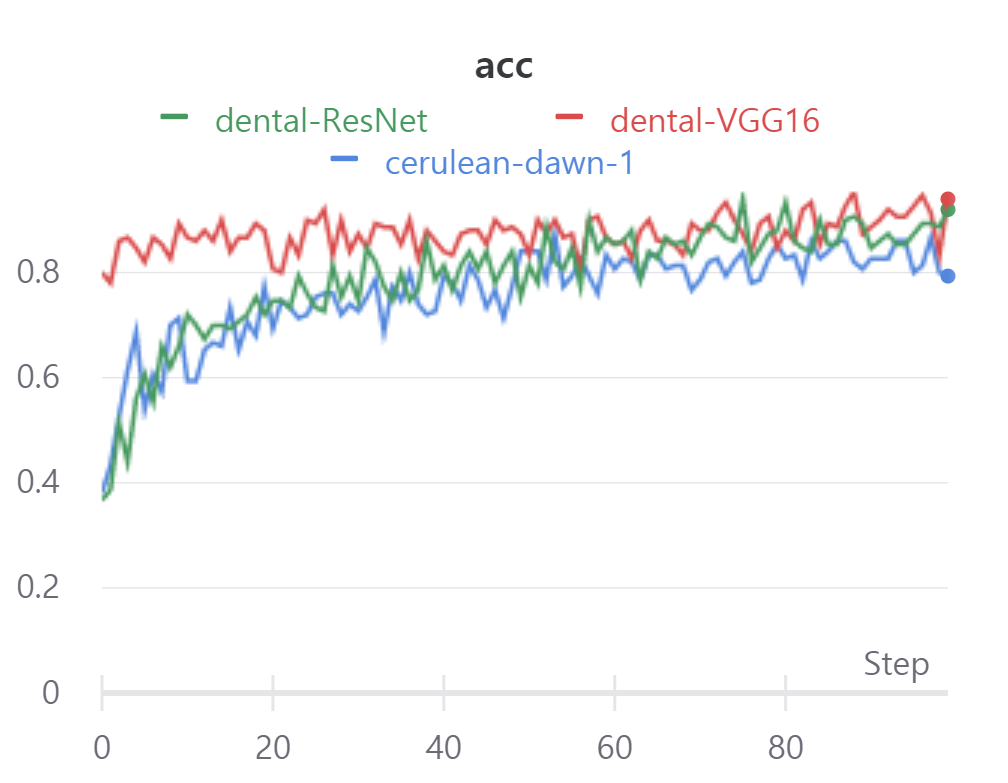
\includegraphics[width=\linewidth]{charts/Section-1-Panel-0-ga735wfu0}
\caption{}
\endminipage\hfill
\minipage{0.49\textwidth}
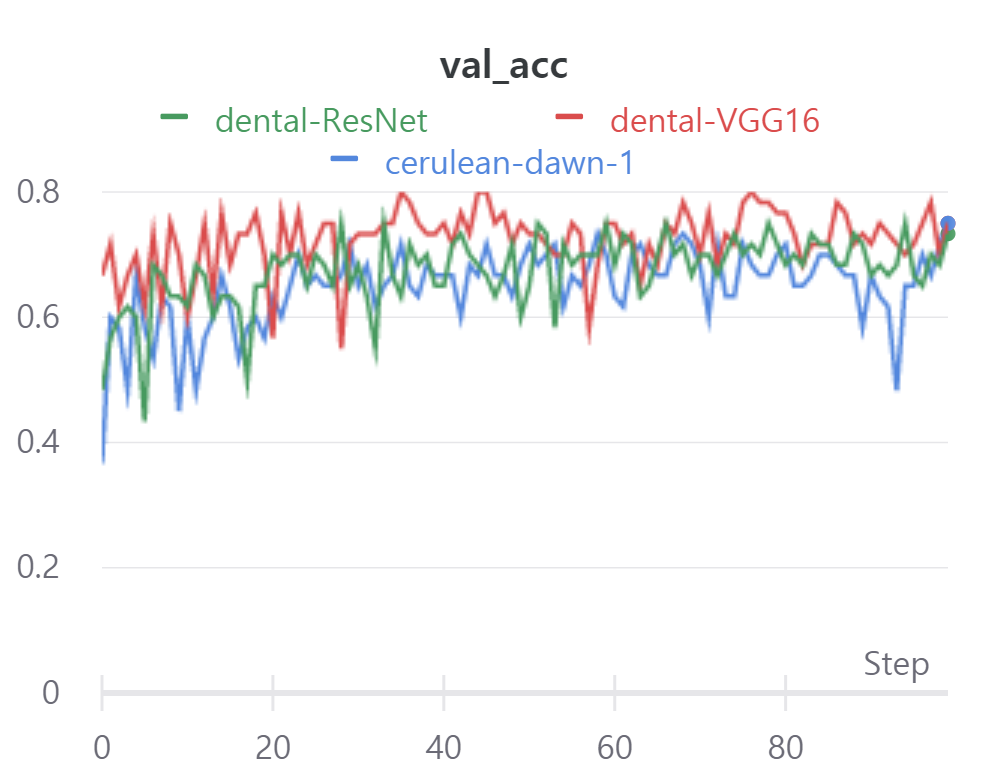
\includegraphics[width=\linewidth]{charts/Section-1-Panel-1-s0lbeggtt}
\caption{}
\endminipage
\end{figure}

\begin{figure}[!htb]
\minipage{0.49\textwidth}
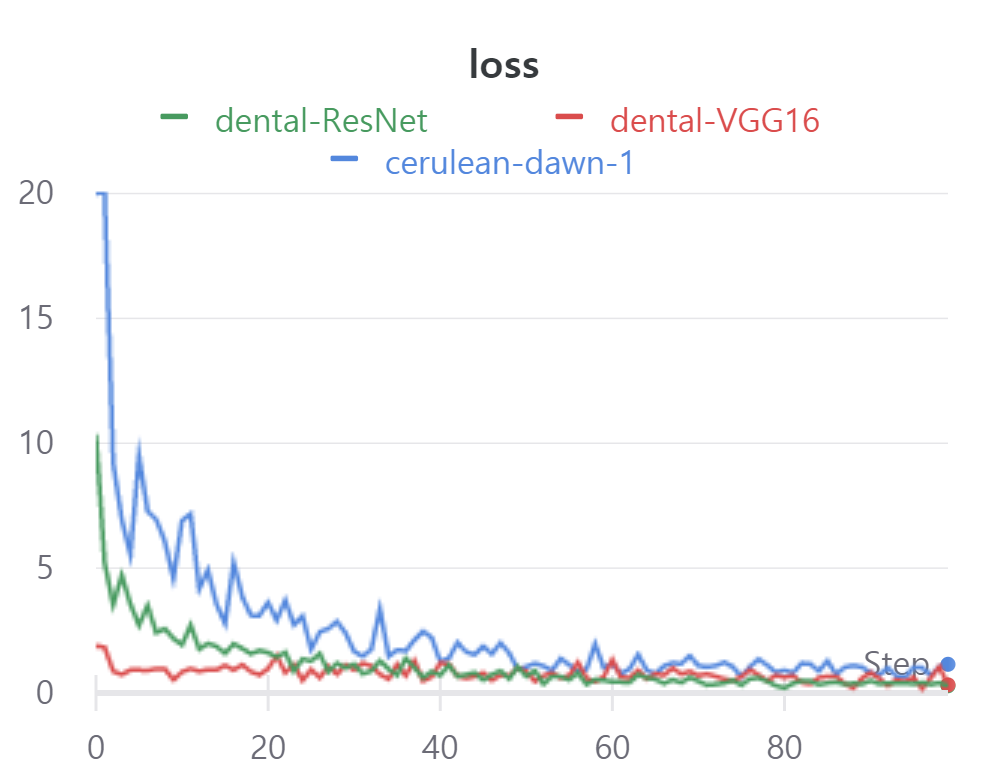
\includegraphics[width=\linewidth]{charts/Section-1-Panel-2-yho4vlz8h}
\caption{}
\endminipage\hfill
\minipage{0.49\textwidth}
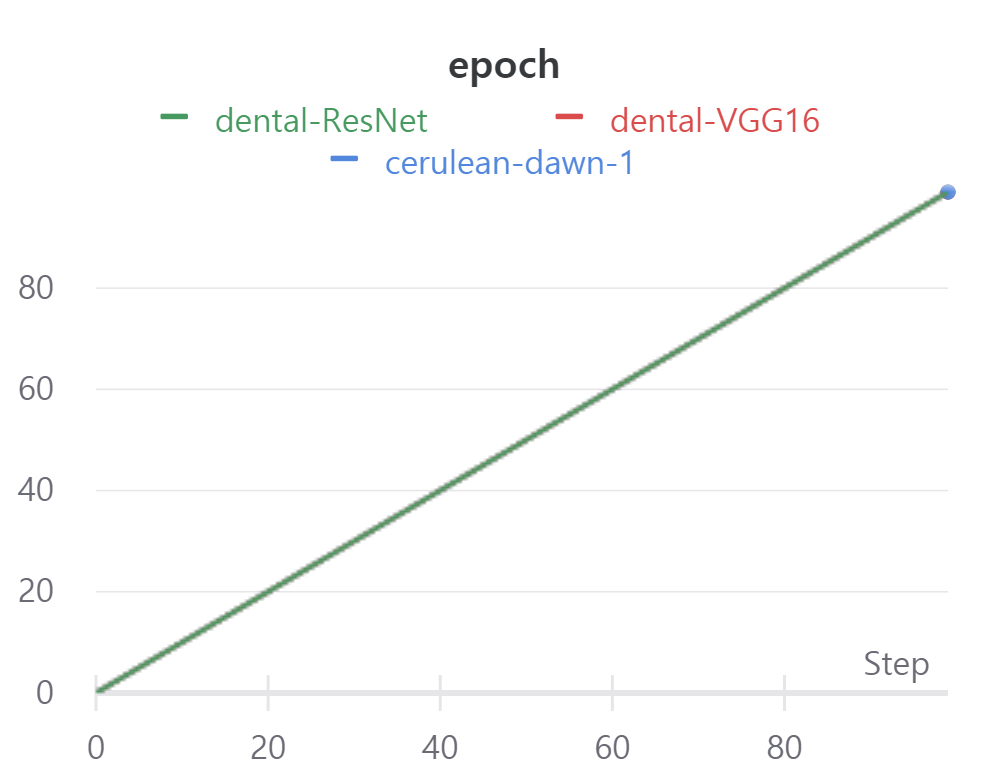
\includegraphics[width=\linewidth]{charts/Section-1-Panel-3-5zvvc0iem}
\caption{}
\endminipage
\end{figure}

\begin{figure}[!htb]
\minipage{0.49\textwidth}
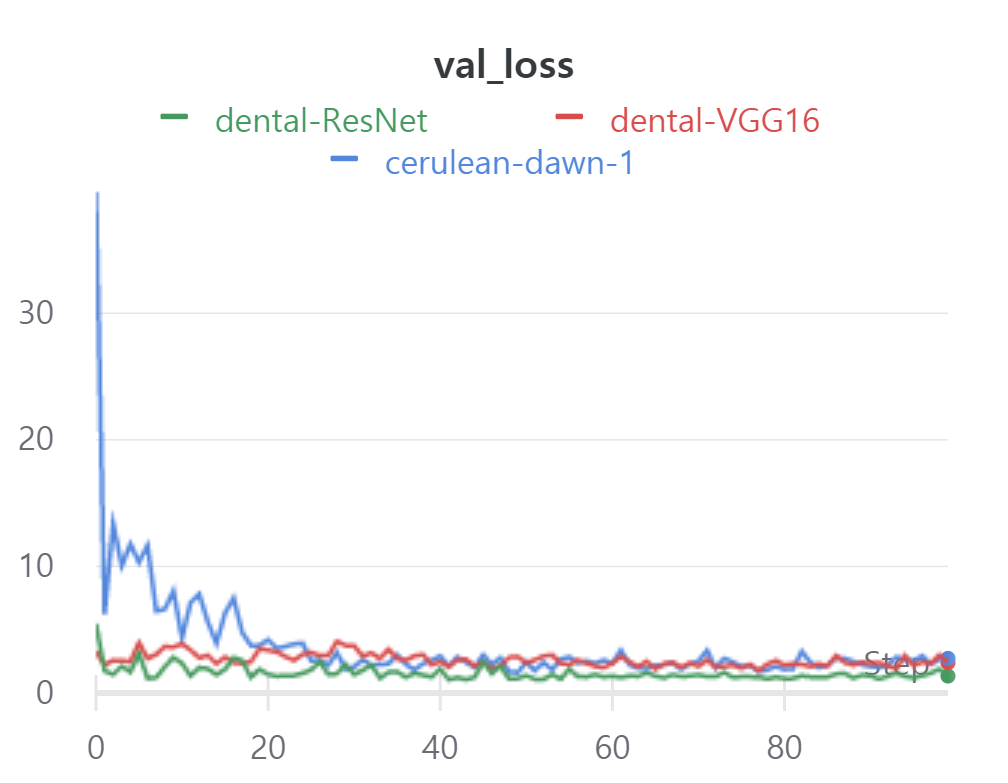
\includegraphics[width=\linewidth]{charts/Section-1-Panel-4-xkb7gowyr}
\caption{}
\endminipage
\end{figure}

\nocite{*}
\bibliographystyle{unsrt}
\bibliography{bibliography}
\end{document}